%----------------------------------------------------------------------
%	DIRC TECHNOLOGY CHAPTER
%----------------------------------------------------------------------
\label{ch:components}
The validation of the key components of the DIRC for an EIC discussed in Chapter \ref{ch:eicdirc} is vital to show that the Geant4 simulation package produces results expected for the real detector. However, due to budget restraints it was not possible to build or otherwise procure a full scale prototype of the envisioned EIC DIRC discussed in Chapter \ref{ch:eicdirc} (e.g. building a DIRC bar and fused silica radiator are outside of the R\&D budget). Instead a series of test bench measurements have been made to validate simulated performance of the new 3-layer lens design, study the radiation hardness of the NLaK33 material, and evaluate the performance of MCP-PMTs in high magnetic field environments.

%----------------------------------------------------------------------
%	3-LAYER LENS OPTICS SECTION
%----------------------------------------------------------------------
\section{Optical Properties of 3-Layer Lens}
\begin{figure}[!htb]
	\centering
	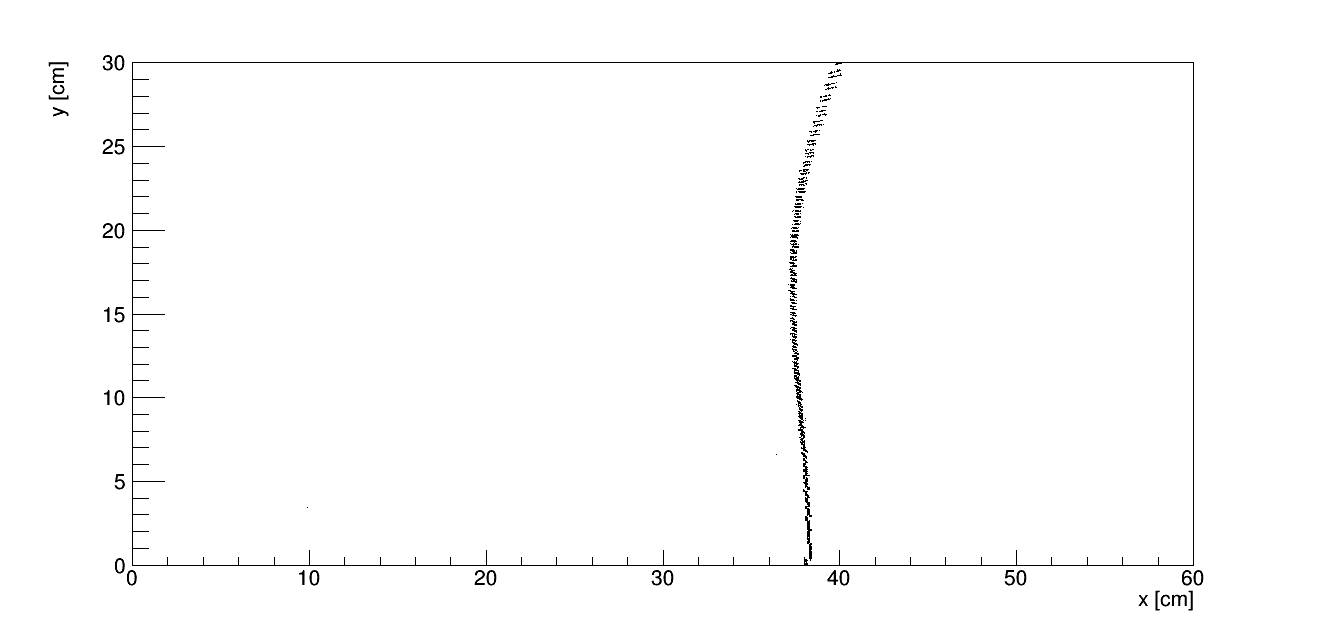
\includegraphics[width=\textwidth]{2D_plane.png}
	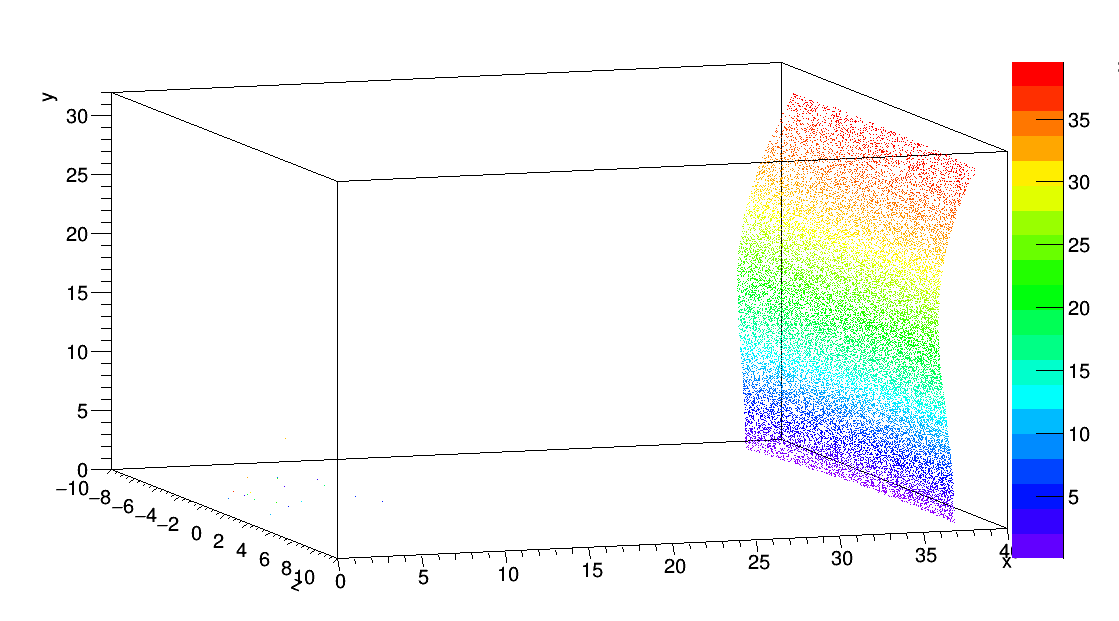
\includegraphics[width=\textwidth]{3D_plane_angle.png}
	\caption{Simulation of the 3-layer lens focal plane with all photons confined to a single plane (top) and the full 3D focal plane (bottom). The color scale corresponds to the initial angle (in degrees) between the laser beams and the lens face. The 3D plane has been constrained to the y/z dimensions of the current expansion volume for the EIC DIRC. The "beams" of photons in the simulation were centered around the center of the lens with a separation of 2 mm.}
	\label{fig:focalplane_sim}
\end{figure}
\begin{figure}[!htb]
	\centering
	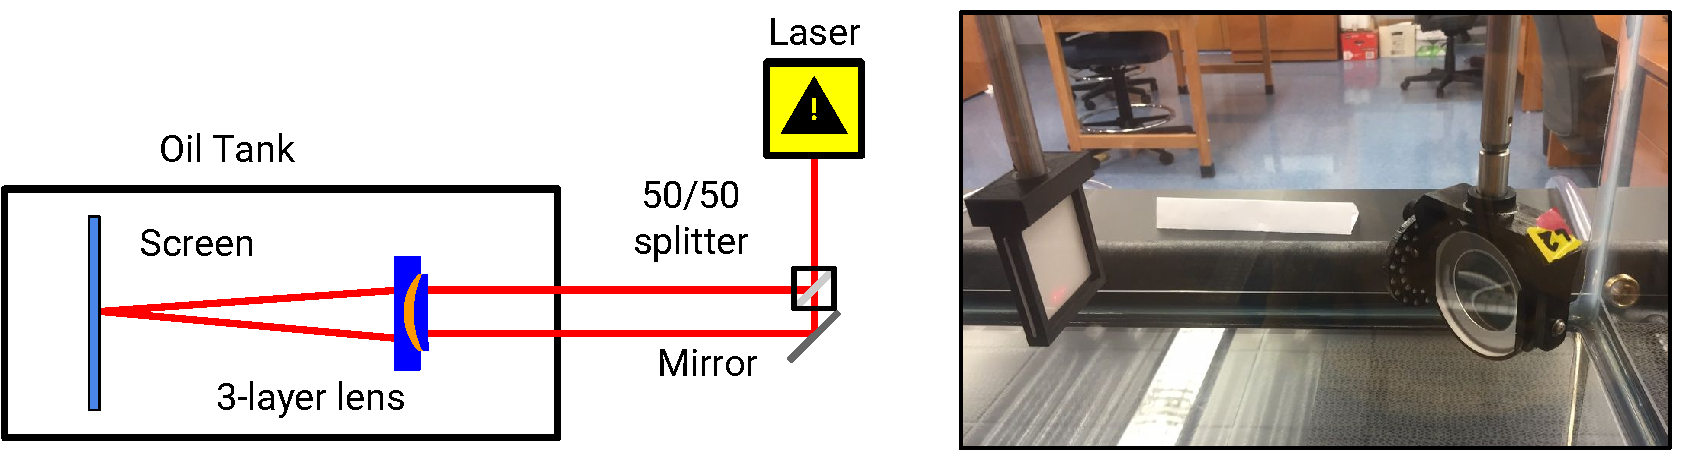
\includegraphics[width=\textwidth]{lens_setup_schematic.pdf}
	\caption{Schematic drawing of the setup built at Old Dominion University for testing the optical properties of the 3-layer lens design (left), and a closeup view of the lens and screen inside the actual setup (right).}
	\label{fig:ODU_setup}
\end{figure}

\begin{figure}[!htb]
	\centering
	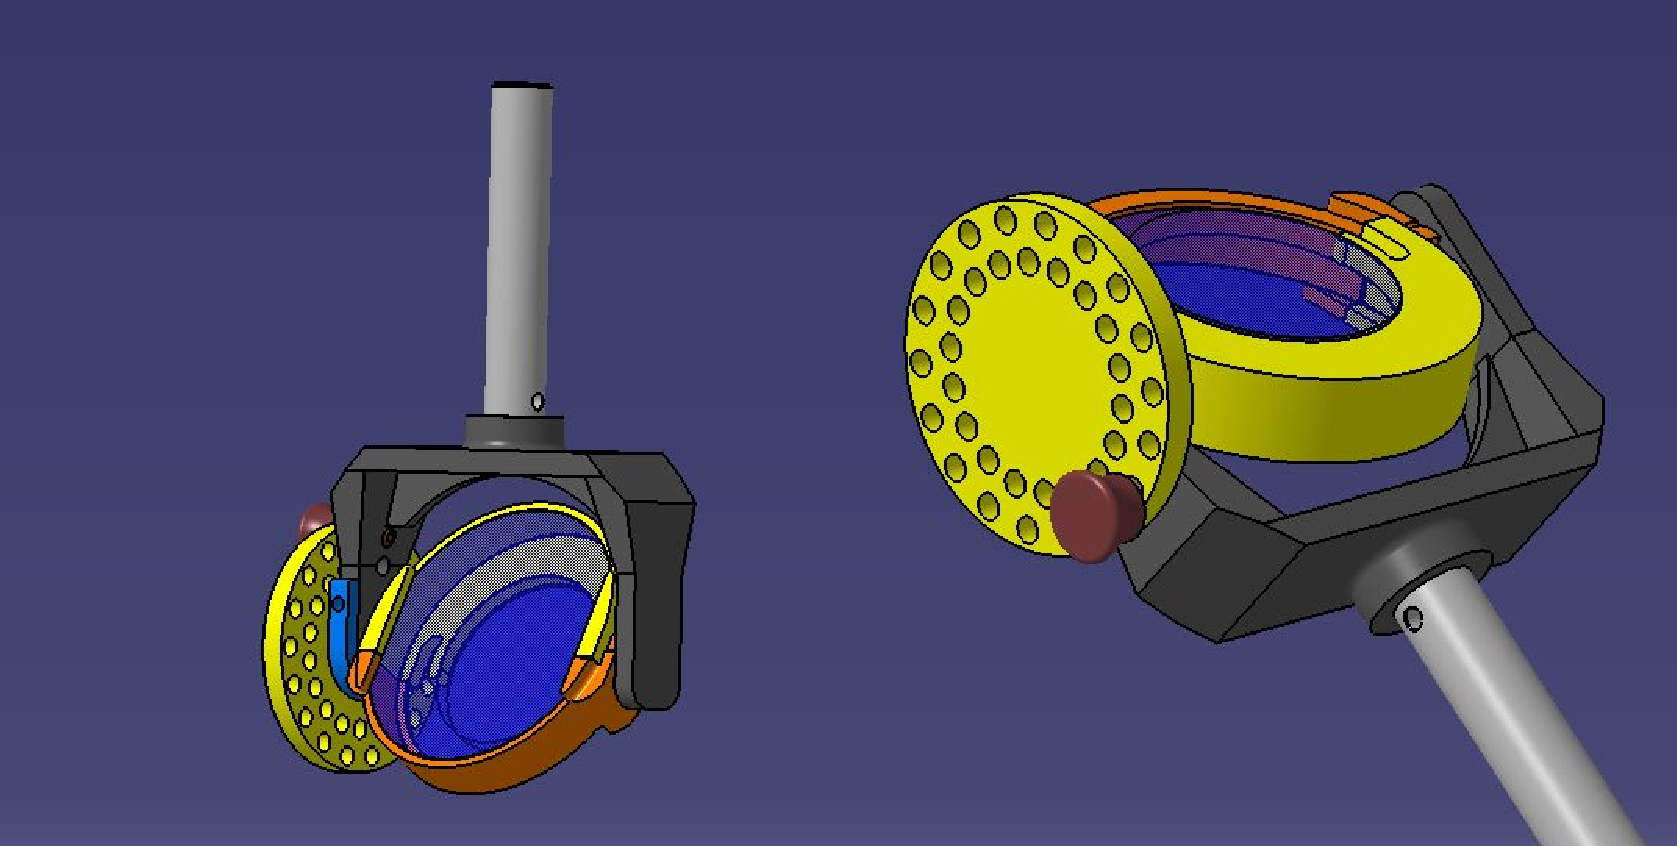
\includegraphics[width=\textwidth]{lens_holder.pdf}
	\caption{CAD drawing of 3-layer lens holder which allows precision rotation in two orthogonal, allowing the full 3D focal plane to be mapped.}
	\label{fig:lens_holder}
\end{figure}

\begin{figure}[!htb]
	\centering
	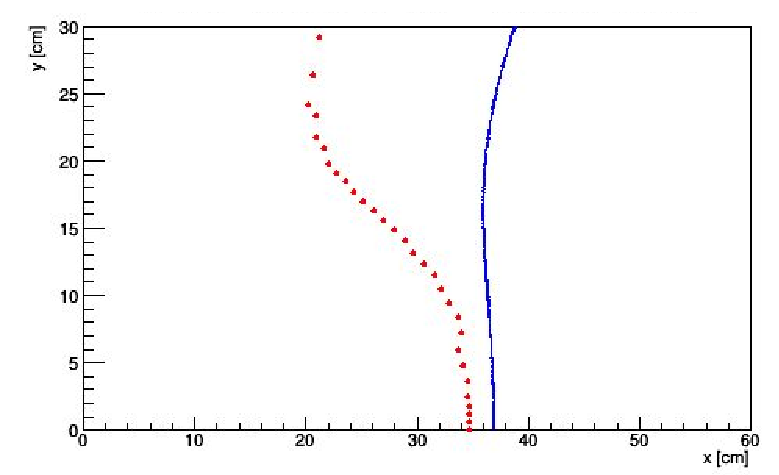
\includegraphics[width=\textwidth]{focalplane_initial.pdf}
	\caption{Initial measurement of the 3-layer lens focal plane using the upgraded green laser (red dots) compared to simulation (blue line).}
	\label{fig:focalplane_initial}
\end{figure}

\begin{figure}[!htb]
	\centering
	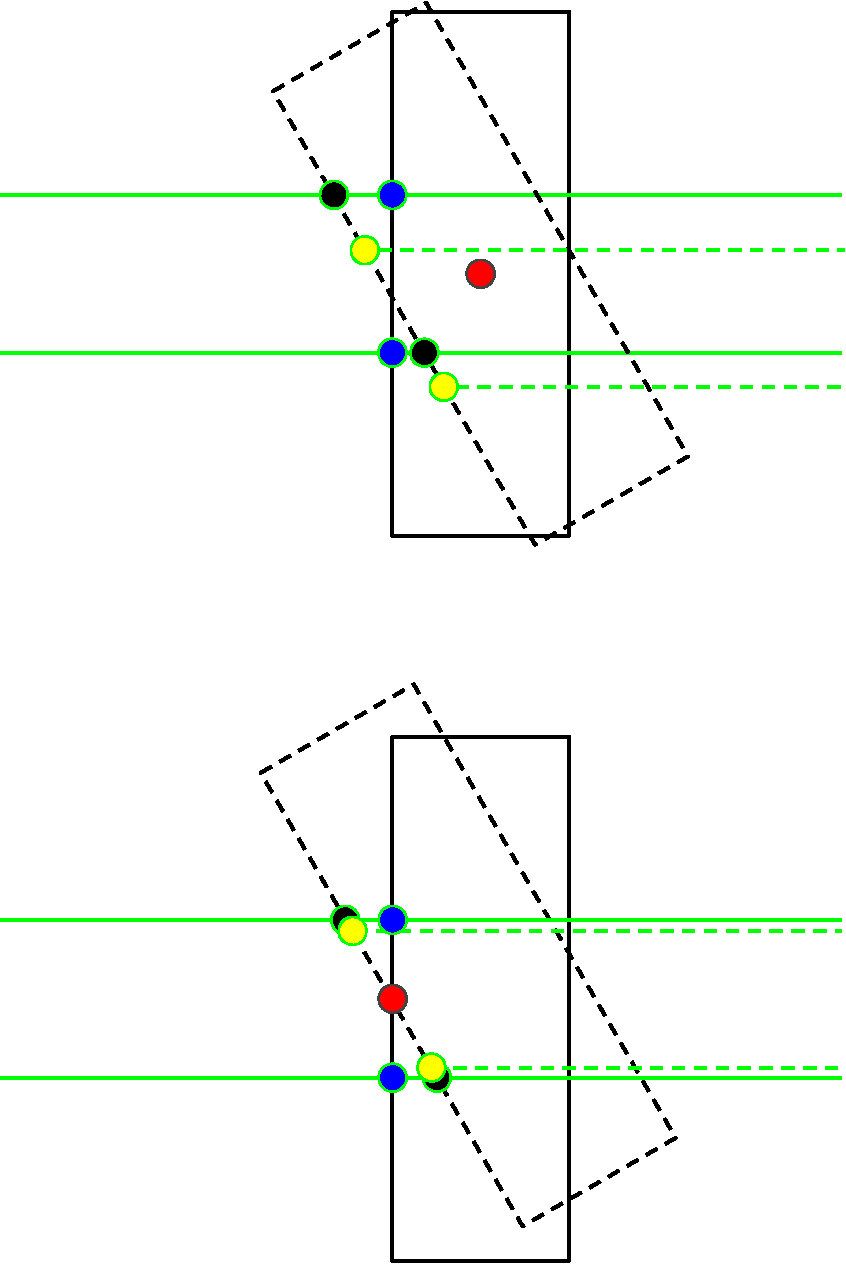
\includegraphics[width=0.43\textwidth]{lens_rotation_point.pdf}
	\caption{Schematic of the discrepancy between beam positions in data (black) and simulation (yellow) in relation to the original beam positions (blue) for a given rotation point (red) at the center (top) of the lens, or at the edge (bottom) of the lens. }
	\label{fig:lens_rotation_point}
\end{figure}

\begin{figure}[!htb]
	\centering
	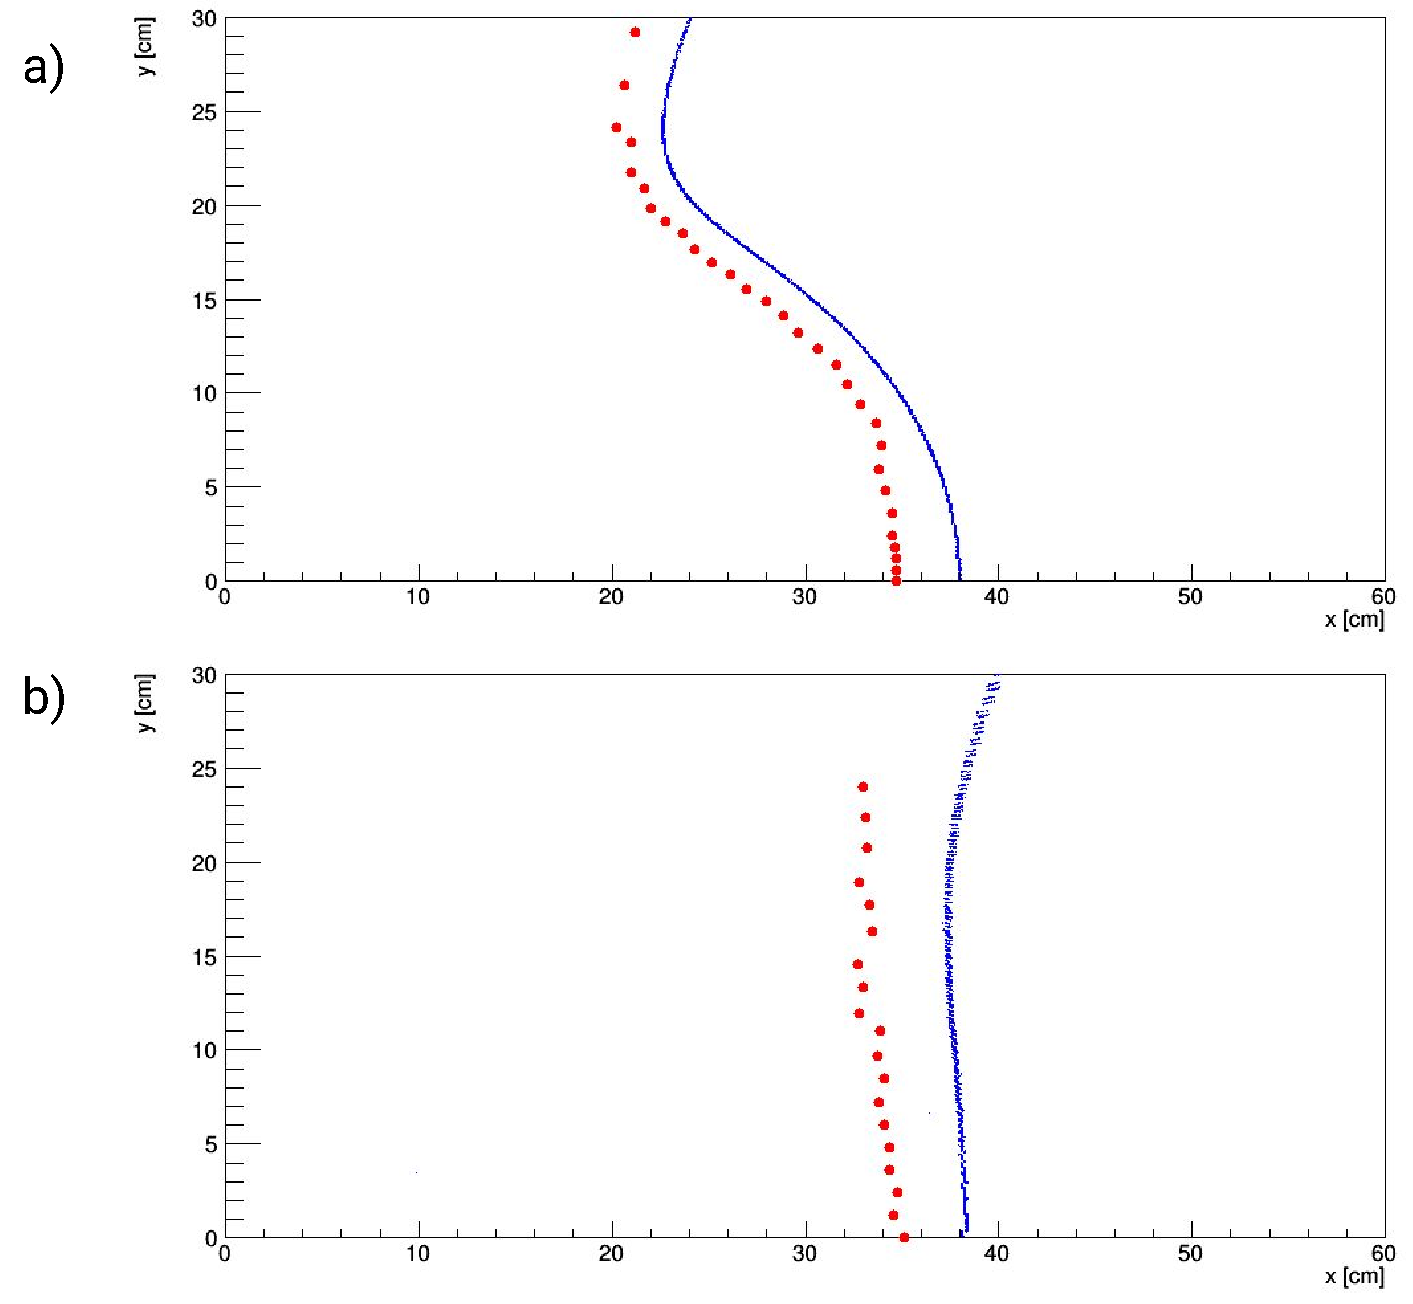
\includegraphics[width=\textwidth]{focalplane_corrections.pdf}
	\caption{Initial measurement of the 3-layer lens focal plane compared to a rotation corrected simulation (a), and a second measurement with a tighter (2 mm) beam configuration and a modified lens holder (b).}
	\label{fig:focalplane_corrections}
\end{figure}

The purpose of the 3-layer lens design is to provide a mostly flat, uniform focal plane across the face of the detector plane. Doing so provides better resolution and hence better performance. A GEANT4 simulation of the nominal (top) and full 3D focal plane (bottom) of the lens are shown in Figure \ref{fig:focalplane_sim}. The 3D plane has been limited to the size of the detector plane anticipated for the EIC DIRC, and the color scale indicates the angle at which photons intersected the front face of the lens. Because only the total focal length is of interest the depth of the expansion volume was limited so that no bounces occurred.

To measure the shape of the focal plane a setup was designed and built, shown in Figure \ref{fig:ODU_setup}, at Old Dominion University in which a laser shines through a 50/50 beam splitter and a mirror to make two beams that are parallel to within 0.5 degrees across roughly 10 meters. The beams then pass through a $30\times40\times60\unit{cm}^3$ glass container filled with mineral oil with a refractive index similar to that of fused silica to simulate the behavior of light passing from bar to lens to expansion volume. The beams are focused through the 3-layer lens, being held in a specially designed holder that allows the lens to be rotated in two planes (Figure \ref{fig:lens_holder}). Finally the beams are focused onto a plastic screen inside the tank that was attached to a track and allowed to slide freely. Due to the relatively low resolution of the human eye the exact point of focus was difficult to measure, so an averaging method was used in which the average of the two points where the beams seem to converge and diverge was taken to be the focal point.

Measurements were initially taken with a 632 nm red helium-neon laser, but the beam spot was too large and very distorted. A 530 nm wavelength green laser with a 1 mm beam spot was then purchased to replace the red laser. Initial results with a 5 mm beam separation are shown in Figure \ref{fig:focalplane_initial}. Obviously there is a large discrepancy in both position and shape of the measured and simulated focal plane. This was rectified by discovering that in the simulation it was assumed that the two beams were entering the lens at fixed points on the lens' face regardless of lens rotation, where as in the experiment the rotation of the lens about it's center causes the beams to shift with respect to the lens face. When rotating at the edge of the lens closest to the laser rather than through the center this difference is negligible, as illustrated in Figure \ref{fig:lens_rotation_point}.

A correction was implemented in the Geant4 simulation to account for the shift of the beam spot during rotation, the results of which can be seen in Figure \ref{fig:focalplane_corrections}a. The beams have since been brought to a 2 mm separation to reduce effects of aberration and a second lens holder was 3D printed to allow for rotation about the edge of the lens. A new round of data was taken and results are shown in Figure \ref{fig:focalplane_corrections}b. This change vastly improved the results of both the simulation from the first measurement and the results of the second, showing that the simulation indeed reproduces very nicely the shape of the focal plane, although the position is still roughly 3 cm too long.

The absolute position of the focal plane can be explained in one of two ways: either the second curved surface of the 3-layer lens has a slightly smaller radius than was requested, or the NLaK33 material has a slightly larger index of refraction than anticipated. Unfortunately measuring either of these quantities is currently unachievable, however the GEANT4 simulation can manipulate both with a high precision. Figure \ref{fig:radius2_shift} shows how decreasing the radius of the second curved surface of the lens by 1.5 mm will bring the focal plane closer to the measured points, but also slightly changes the shape of the focal plane. Figure \ref{fig:NLaK_shift} shows that a very small increase in the refractive index of the NLaK33 material matches the data quite nicely and without distorting the original shape of the plane.

Despite the irregularity between the measured and ideally simulated focal plane lengths, the overall shape is still very consistent with a flat detector plane. The radii of the two layers must be optimized for the EIC design. Procurement of a new lens is underway to be used in an upcoming test beam at CERN in 2017.


\begin{figure}[!htb]
	\centering
	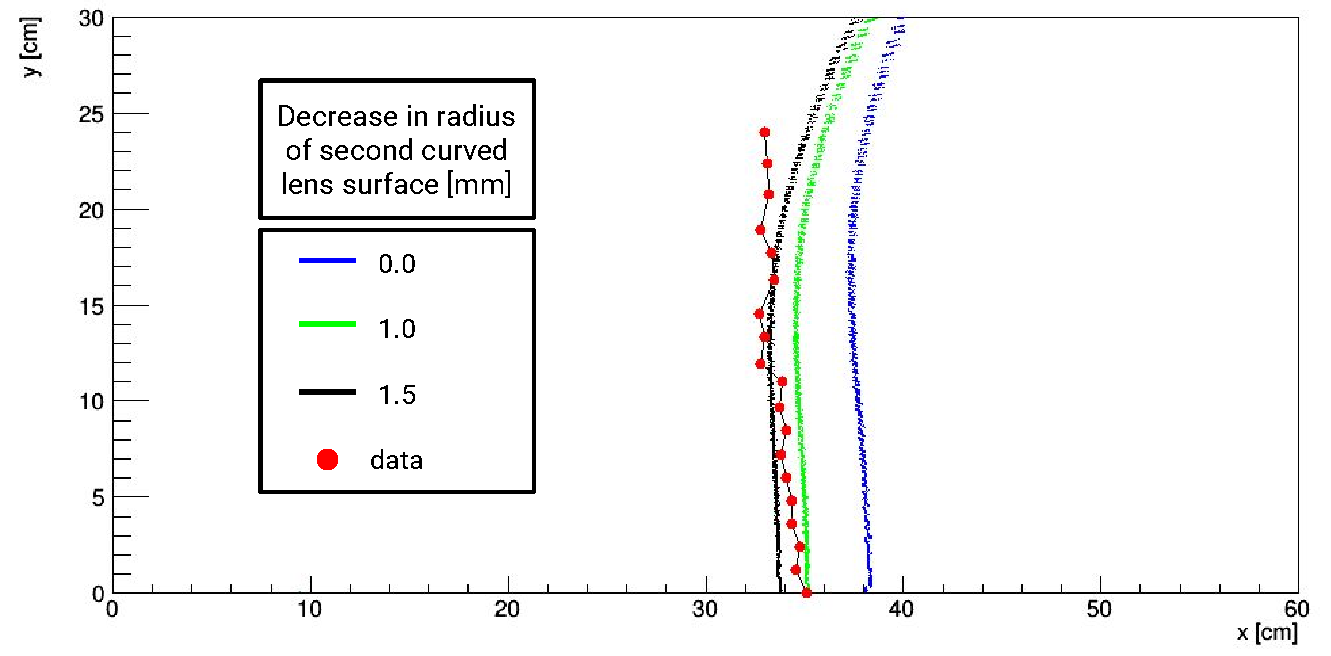
\includegraphics[width=\textwidth]{radius2_shift.pdf}
	\caption{Decreasing the radius of curvature of the second curved surface of the 3-layer lens shifts the focal plane towards the measured results, but also slightly changes the shape of the focal plane. A shift of 1.5 mm, or approximately 5\%, is sufficient to roughly agree with the data.}
	\label{fig:radius2_shift}
\end{figure}

\begin{figure}[!htb]
	\centering
	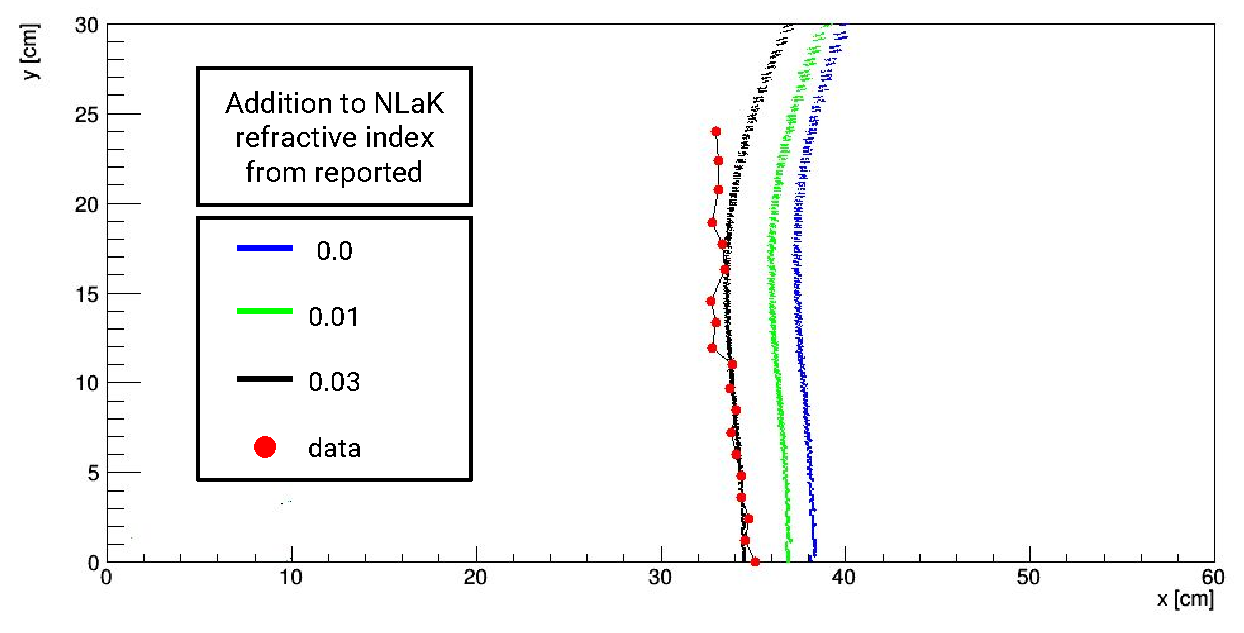
\includegraphics[width=\textwidth]{NLaK_shift.pdf}
	\caption{Increasing the refractive index of the NLaK33 material shifts the focal plane towards the measured results while keeping the overall shape of the plane intact. An increase of 0.03, or approximately 2\%, is sufficient to follow the measured data.}
	\label{fig:NLaK_shift}
\end{figure}
%----------------------------------------------------------------------
%	NLAK33 RAD HARDNESS SECTION
%----------------------------------------------------------------------

\section{Radiation Hardness of NLaK33}
Fused silica, which is used for most of the optical components in all current DIRC designs, was already extensively tested in the BaBar and PANDA experiments \cite{RadHardness} and has proven to be radiation hard up to several hundred kRad with little to no loss of transmission. The determination of the radiation hardness of NLaK33 is an important study for the EIC R\&D program. 

The irradiation of a pure sample of NLaK33 material was performed at Catholic University of America in a Faxitron CP-160 Cabinet X-Radiator System \cite{XRayCabinet} (Figure \ref{fig:x-ray_setup}a). The cabinet allows for a minimum of 6 second X-ray exposure. Photon energy was set to 160 keV with a 6.2 mA current for all exposures of the NLaK33 sample.

A RaySafe ThinX RAD dosimeter \cite{Dosimeter}, shown sitting on the X-ray cabinet shelf in Figure \ref{fig:x-ray_setup}b, was used to measure the radiation dose being delivered to the sample. Unfortunately the exposure time of the dosimeter is limited to less than 10 seconds, so the shortest time setting on the X-ray cabinet was used. This exposure time of 6 seconds was found to be closer to 7.5 seconds by the dosimeter due to rise and fall time of the source. This shortest exposure time consistently gave readings of 81.4 Rad. The dosimeter has a circular active area of $706.9\unit{mm}^2$ while the side of the NLaK33 sample that was exposed to the source has an area of $8\times28\unit{mm}^2$, so the relative dose delivered to the sample is approximately 25 Rad.

To measure the transmission of the sample a LAMBDA 950 UV/Vis/NIR Spectrophotometer \cite{Monochromator} (Figure \ref{fig:monochromator_setup}a), refereed to from here on as a monochromator, was used. The monochromator has a dynamic range between 175 - 3,300 nm wavelength in 1 nm steps. The sample of NLaK33 was held in place using an optics stand (Figure \ref{fig:monochromator_setup}b) to make sure measurements were consistent and reproducible. Measurements of the transmission of the sample were taken between each set of radiation exposures. The transmission of sample of fused silica was also tested between each radiation exposure of the NLaK33 sample, but was only used as a control sample and was found to be quite stable.

Because it was not clear exactly what percentage of the total dose read by the dosimeter was from the warm up and cool down of the cabinet it was decided that the best approach for exposure of the sample was to do multiple steps of the 6 second exposure time and record the accumulated dose in this manner. The first exposure was 4 intervals for a total of 100 Rad. After this measurement it was noticed that there was already a roughly 2\% drop in the transmission of the sample at 420 nm wavelength, so steps of 50 Rad were taken for the next several measurements. Results are shown in Figure \ref{fig:transmission_measurements}. After 700 Rad of dose it was clear that there was a linear correlation between accumulated dose and loss in transmission, so it was decided that 100 Rad steps could again be taken.

\comment{results plot is only a placeholder for now, need to remake plots in ROOT so they look a little nicer}

\begin{figure}[!htb]
	\centering
	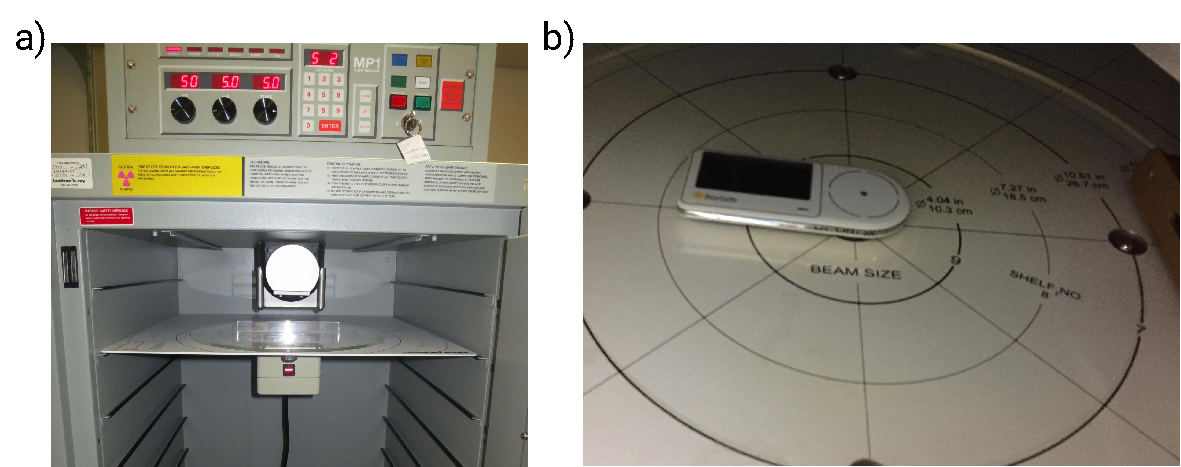
\includegraphics[width=\textwidth]{x-ray_setup.pdf}
	\caption{The Faxitron CP-160 Cabinet X-Radiator System (a) used to irradiate the NLaK33 sample with 160 keV photons at 6.2 mA current for 6 second intervals, and the RaySafe ThinX RAD Dosimeter (b) sitting on one of the X-ray cabinet shelves.}
	\label{fig:x-ray_setup}
\end{figure}


\begin{figure}[!htb]
	\centering
	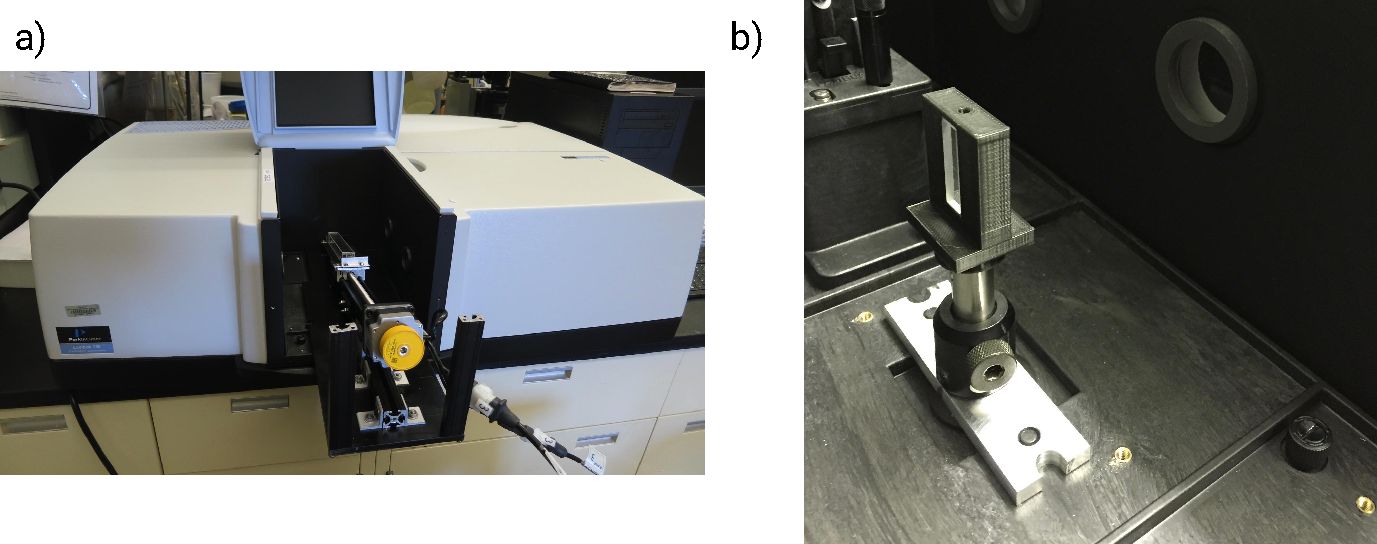
\includegraphics[width=\textwidth]{monochromator_setup.pdf}
	\caption{The LAMBDA 950 UV/Vis/NIR Spectrophotometer (a) and a closeup view of the NLaK33 sample being held in position by the optics stand (b).}
	\label{fig:monochromator_setup}
\end{figure}

\begin{figure}[!htb]
	\centering
	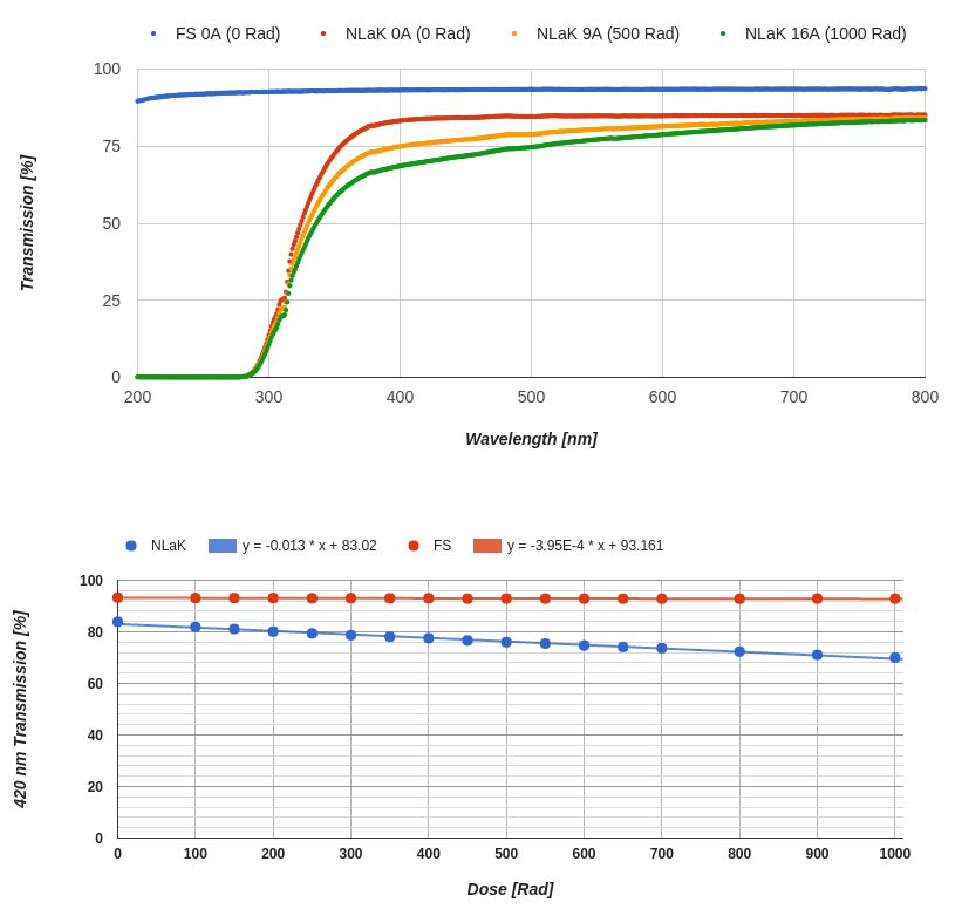
\includegraphics[width=\textwidth]{transmission_measurements.pdf}
	\caption{The top plot shows the transmission of the control sample of fused silica (blue) and the transmission of the NLaK33 sample after 0 (red), 500 (orange), and 1000 (green) Rad doses across a range of 200-800 nm wavelength. The bottom plot shows only the transmission of the two samples at 420 nm wavelength as a function of the dosage for fused silica (red) and NLaK33 (blue). The circles are the measured data points while the solid lines are a linear fit describing the data. After the first 700 Rad of dose it was clear that there was a linear relationship between dose and transmission loss and so 100 Rad steps were used afterwards.}
	\label{fig:transmission_measurements}
\end{figure}

%----------------------------------------------------------------------

%	HIGH-B TESTS SECTION
%----------------------------------------------------------------------

\section{Performance of MCP-PMTs in High Magnetic Field}
The limiting space requirements of the EIC DIRC design, as mentioned in Chapter \ref{ch:eicdirc}, places a unique set of requirements on the DIRC readout sensors. In order to achieve the desired single photon resolution while maintaining a sufficiently sized expansion volume the sensors, and therefore the pixels, must be compact. Furthermore, due to the positioning of the readout plane being inside the large field of the solenoid magnet (see Figure \ref{fig:jleic_layout}) these sensors must also have a high tolerance to magnetic fields, both in magnitude (up to 3 T or higher), non-uniformity, and orientation. Ordinary photomultiplier tubes (PMTs) are not an option due to their susceptibility to magnetic fields, being affected by fields as small as 0.5 Gauss \cite{PMT_magnet}. Silicon photomultipliers (SiPMs) are attractive due to their very compact size and their resistance to magnetic fields up to 4 T \cite{SiPM_characterization}. However, the inherent background, or dark count, of SiPMs is very large, on the order of MHz \cite{SiPM_characterization}. Because a DIRC detector only expects 60 photons per event at most this level of background is far too large for usability. With these requirements in mind the best option for an EIC DIRC detectors is the use of micro-channel plate photomultiplier tubes (MCP-PMTs) (Figure \ref{fig:MCP_schematic}). The dark count of MCP-PMTs is on the order of kHz \cite{MCPPMT_darkcount}, which is much more acceptable compared to SiPMs. MCP-PMTs also have a much higher resistance to external magnetic fields than traditional PMTs due to the small pore size, with studies being done up to 2 T \cite{MCPTest1}, \cite{MCPTest2}, \cite{MCPTest3}, \cite{MCPTest4}, \cite{MCPTest5}, \cite{MCPTest6}. The tests described below are the first to study the effects of fields as large as 5 T on MCP-PMTs.

\begin{figure}[!htb]
	\centering
	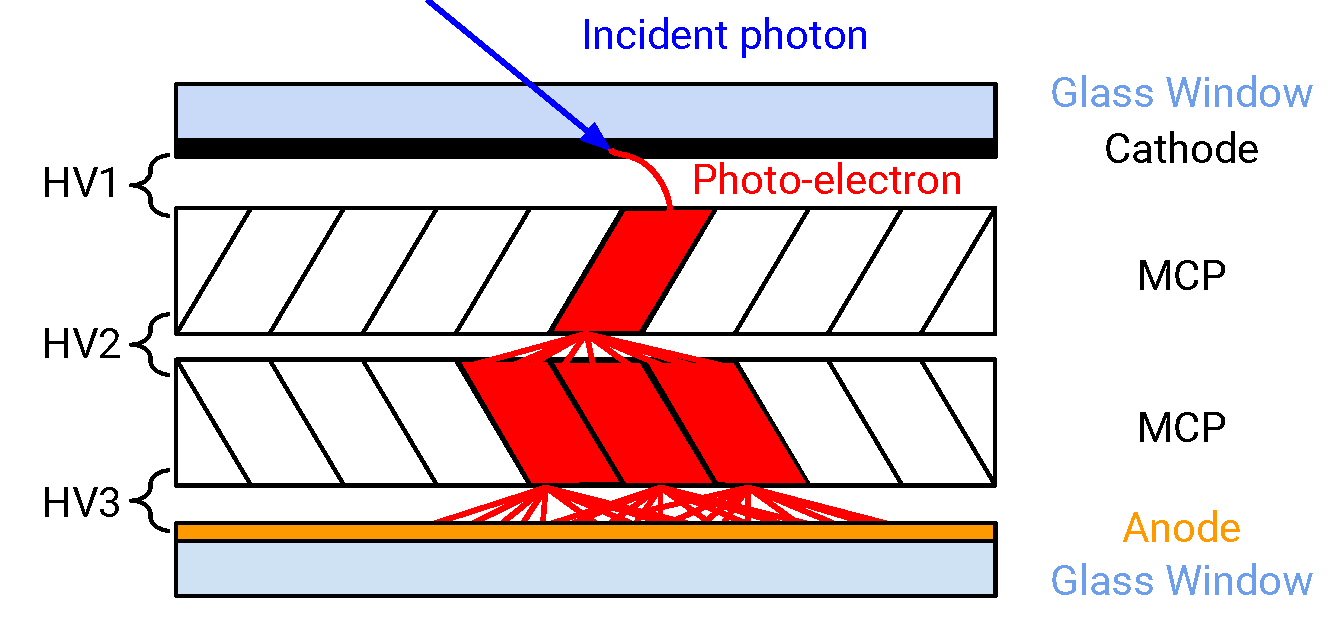
\includegraphics[width=\textwidth]{MCP_schematic.pdf}
	\caption{Schematic of the Micro-channel Plate photo-multiplier tube (MCP-PMT) concept. A cathode and anode sandwich two conducting plates with micrometer-sized channels (MCP), and a high voltage difference (HV1, HV2, HV3) between every two components. The channels, or pores, of the two MCPs are aligned in a chevron pattern. An incident photon (blue) strikes the cathode, producing a photo-electron (red). That electron is accelerated through the potential difference between the cathode and first MCP (HV1) before striking the inside of one channel. This creates the same effect as an electron striking the dynode of a typical PMT, resulting in an avalanche of photo-electrons that emerge out of the other side of the first MCP. These electrons are again accelerated through a second potential difference (HV2) before repeating the process in the second MCP. Finally, the copious photo-electrons exit the second MCP, are accelerated through a final potential difference (HV3), and are collected on the anode. This design is both much more compact, more resistant to magnetic fields compared to traditional PMTs, and has less timing jitter. }
	\label{fig:MCP_schematic}
\end{figure}

In the fall of 2014 two MCP-PMTs were tested at Jefferson Lab \cite{HighB_DIRC2015}, a PHOTONIS PP0365G \cite{PHOTONIS} and a Photek PMT210 \cite{Photek}. The FROST  superconducting solenoidal magnet, with a field tunable up to 5 T with a cylindrical bore diameter of 12.7 cm and a length of 76.2 cm, was used for testing \cite{JLab_FrozenTarget}. The central field of the magnet, while quite large, is also very homogeneous, with an inhomogeneity of less than $5\times10^{-5}$ over a cylindrical volume with a diameter of 1.5 cm and a length of 5 cm. The sensors that were tested were held in place at the center of the magnet using a custom-built, non-magnetic, light-tight cylindrical dark box, as shown in Figure \ref{fig:highB_magnet}. Inside the dark box the sensor was held in place by a turn table that allowed for rotation around a vertical axis as well as a horizontal axis (the Y(Y') and Z(Z') axes in Figure \ref{fig:highB_schematics} respectively). The range of the polar angle $\theta$ was dependent on the size of the sensor being measured as well as the signal and high-voltage cables connected to the back of the sensor. A cart allowed the sensor to move relative to the dark box for precise positioning at the center of the magnet.

A pulser-driven LED was used to illuminate the MCP-PMTs with 470 nm photons. An optical fiber was used to transmit the photons to the dark box and a diffuser installed inside the dark box cap was used to illuminate the entire face of the sensor with nearly constant intensity and 10 ns wide pulses at 30 kHz. The sensor signal output was then amplified using a 200-times preamplifier and used as input to a flash analog-to-digital converter (fADC). The fADC was then read out by our data acquisition system (DAQ).The pulser was also used as the trigger signal for the fADC, as shown in the chart in Figure \ref{fig:highB_schematics} (right).


\begin{figure}[!htb]
	\centering
	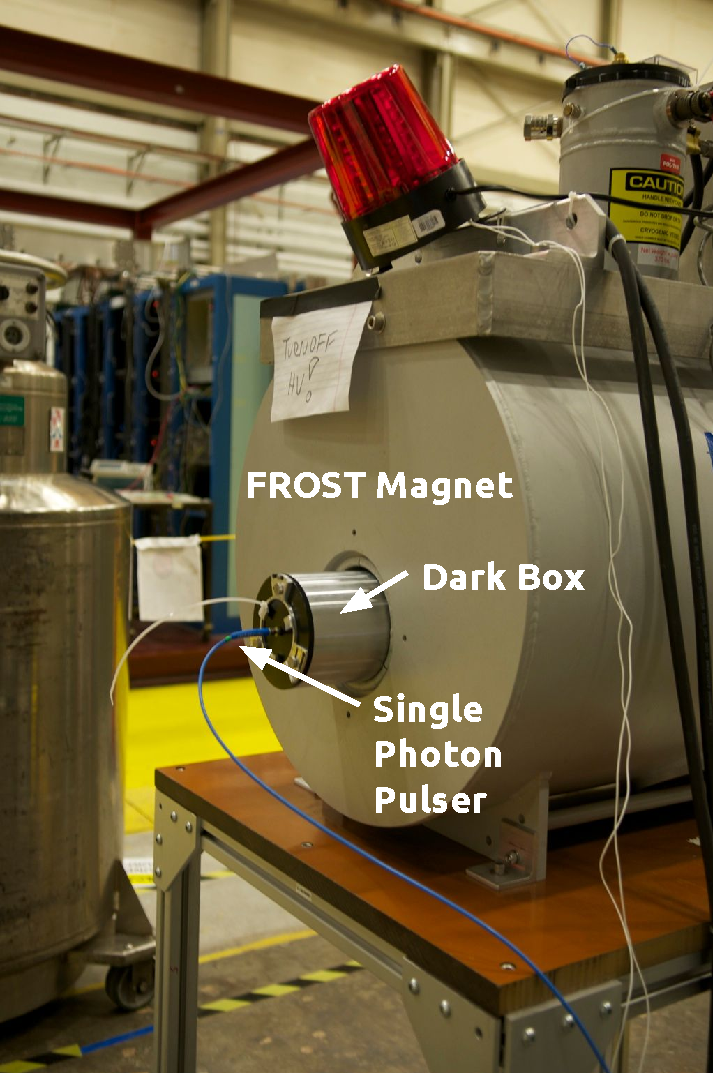
\includegraphics[width=0.4\textwidth]{highB_magnet.pdf}
	\caption{The FROST superconducting magnet with the dark box placed in the bore.}
	\label{fig:highB_magnet}
\end{figure}

\begin{figure}[!htb]
	\centering
	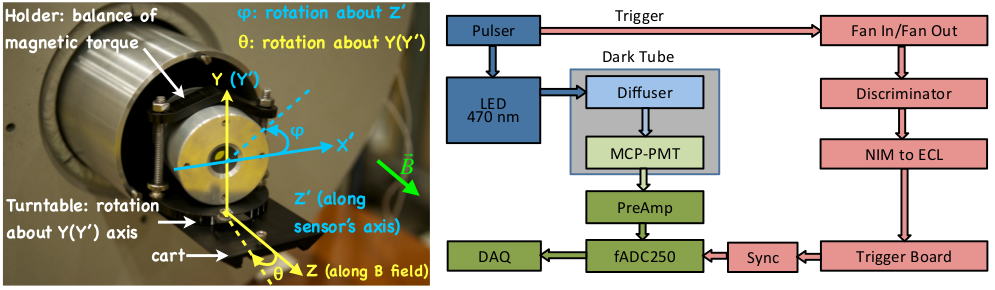
\includegraphics[width=\textwidth]{highB_schematics.png}
	\caption{Left: A closeup of the dark box showing the Photek PMT210 being held in place by the turn table. This setup allows the MCP-PMT to be rotated around both the horizontal Z(Z') axis as well as the vertical Y(Y') axis (with respect to the floor). The rotation about the Y(Y') and Z(Z') axes are described by the polar angle $\theta$ and azimuthal angle $\phi$ respectively. The magnetic field is parallel to the central axis of the dark box. Right: A flowchart of the readout used for testing. The photocathode is exposed to single 470 nm photons to produce photoelectrons, with a large voltage difference between the anode and cathode used to create an avalanche. The total charge is collected on the anode, amplified by a preamplifier, and digitized by an fADC and read out by a DAQ. \cite{HighB_DIRC2015} }
	\label{fig:highB_schematics}
\end{figure}

\begin{figure}[!htb]
	\centering
	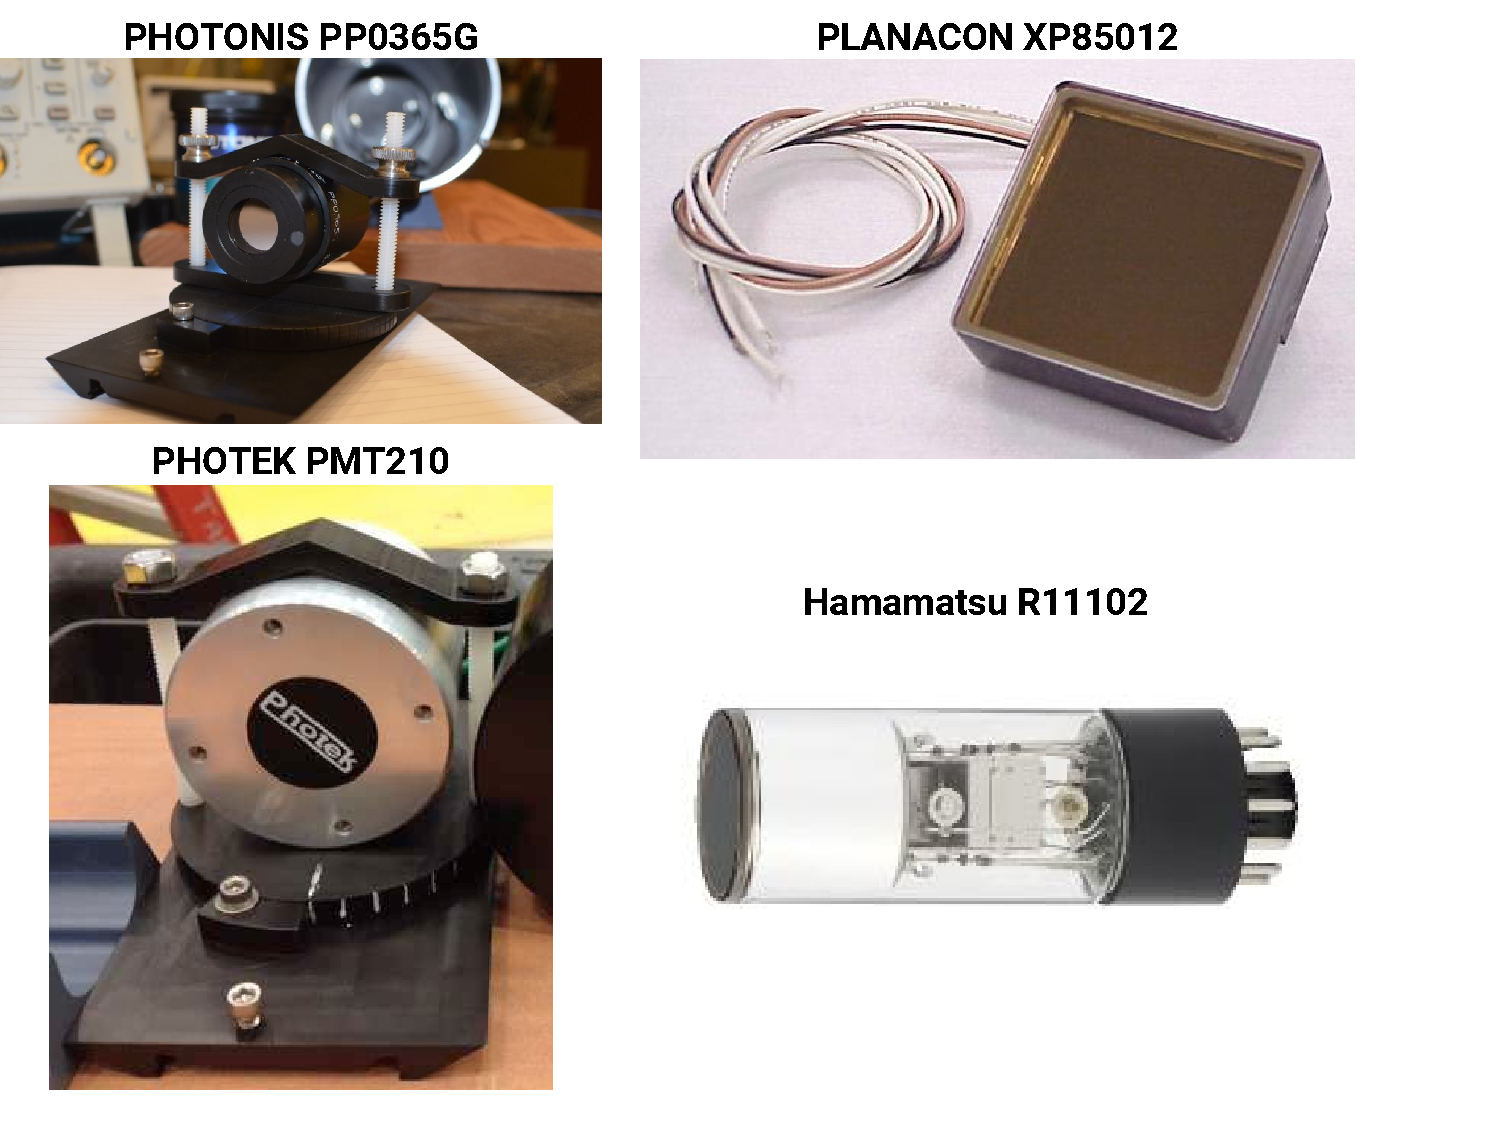
\includegraphics[width=\textwidth]{highB_sensors.pdf}
	\caption{The FROST superconducting magnet with the dark box placed in the bore.}
	\label{fig:highB_sensors}
\end{figure}